\documentclass{standalone}
\usepackage{tikz}
\usetikzlibrary{calc}

\begin{document}
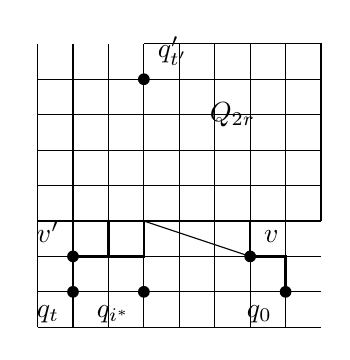
\begin{tikzpicture}[
    dot/.style={circle,fill,inner sep=1.5pt,outer sep=0pt},
    scale=0.45
  ]
  
  % Draw the grid
  \foreach \i in {0,...,7} {
    \draw (\i, 0) -- (\i, 8);
    \draw (0, \i) -- (8, \i);
  }
  
  % Draw Q_{2r}
  \draw (3, 8) -- (8, 8) -- (8, 3);
  \node at (5.5, 6) {$Q_{2r}$};
  
  % Draw the cells and dots
  \node[dot, label=below left:$q_0$] at (7, 1) {};
  \node[dot, label=above right:$v$] at (6, 2) {};
  \node[dot, label=above left:$v'$] at (1, 2) {};
  
  \draw[thick] (1, 7) -- (1, 3) -- (3, 3);
  \node[dot, label=above right:$q'_{t'}$] at (3, 7) {};
  
  % Highlighted cells
  \draw[thick] (1, 2) -- (1, 3);
  \draw[thick] (1, 2) -- (2, 2) -- (2, 3);
  \draw[thick] (2, 2) -- (3, 2) -- (3, 3);
  \draw[thick] (6, 2) -- (7, 2) -- (7, 1);
  \draw[thick] (6, 2) -- (6, 3);
  
  % Paths
  \node[dot, label=below left:$q_t$] at (1, 1) {};
  \node[dot, label=below left:$q_{i^*}$] at (3, 1) {};
  \draw (1, 1) -- (1, 2);
  \draw (3, 1) -- (3, 3);
  
  % Lines from v and v' to q'_{t'}
  \draw (6, 2) -- (3, 3);
  \draw (1, 2) -- (1, 3);
  
\end{tikzpicture}
\end{document}